\section{Evaluation}
\label{eval}

%Evaluation section...
%
%Length: 3-4 pages (graphs take a lot of space!)
%
%Tell reader what to expect.
%
%Eval is "proof" that your design is good.
%MATCH eval goals with design goals.
%
%Eval section is easier to write, but longest one to produce
%results for.  Whereas design section has complex structure, eval
%is more 'flat'.
%
%Structure:
%
%1.  list eval goals, should match design goals
%
%2.  briefly list how you plan to prove those goals.
%
%3.  describe your testbed: h/w + s/w platform to run tests on.
%Give enough detail so it can be reproduced by ANYONE.
%
%4.  describe your benchmarks in detail:
%
%(4a) Micro benchmarks: test specific feature (e.g., read or
%write performance).  Usually u-bench are designed to highlight
%worst/best case behavior of your system.  Be to list both best
%and worst.
%
%(4b) Macro benchmarks (general purpose benchmarks): test whole
%system (e.g., run a Web server exerciser, or TPC for database).
%
%Some tests should compare YOUR system to past systems, or a
%"before and after" comparison.
%
%For every possible variable in your system, design a set of
%independent tests (re: compression study's dimensions).  Justify
%need to vary each variable (the more variables, the more
%experiments you have to run).
%
%5.  Describe your benchmarking methodology
%
%Statistical stability: how many times you run each test? do you
%compute standard deviations, half-width intervals (for student-t
%distribution), RMS, or other metric of stability?  Say how many
%times you ran each test, and what were the stability metrics.
%
%Ex."we ran every test at least 10 times, and computed the
%standard deviation as a percentage of the mean.  In all cases,
%the percentage was less than 5\%, unless otherwise noted."
%
%6.  List every benchmark result, for each test
%
%(a) a graph or table or other figure, plus caption.
%(b) followed by an explanation of the figure: say what one sees
%    in the figure, then explain WHY it is so.
%
%7.  Optional: if eval section longer than usual, end it with a
%one-paragraph summary of eval results.

\begin{figure*}[ht]
    \centering
    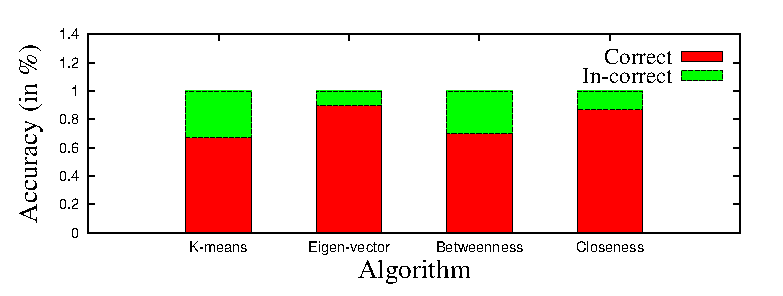
\includegraphics[width=1\textwidth]{figures/social-result_arvind.eps}
    \caption{Comparison of accuracy of algorithms, based on validated result data from Arvind.}
    \label{fig:social-result-arvind}
\end{figure*}

\begin{figure*}[ht]
    \centering
    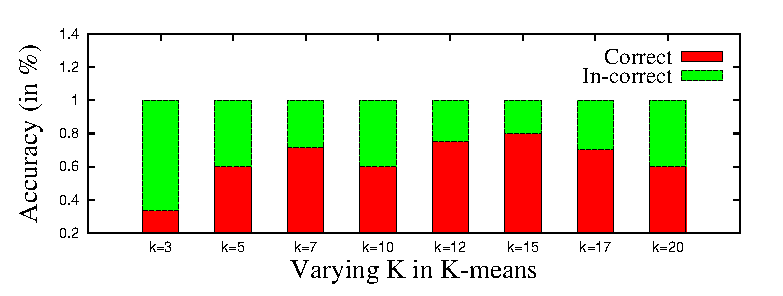
\includegraphics[width=1\textwidth]{figures/social-result_arvind_kmeans.eps}
    \caption{Comparison of accuracy of K-means on varying k, based on validated data from Arvind.}
    \label{fig:social-result-arvind-kmeans}
\end{figure*}

\begin{figure*}[ht]
    \centering
    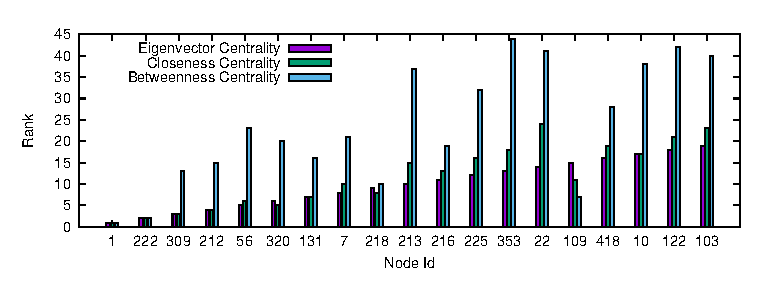
\includegraphics[width=1\textwidth]{figures/social-result_eigen.eps}
    \caption{Rank comparison for top 20 nodes ranked on eigenvector centrality with other centrality scores.}
    \label{fig:social-result-eigen}
\end{figure*}

\begin{figure*}[ht]
    \centering
    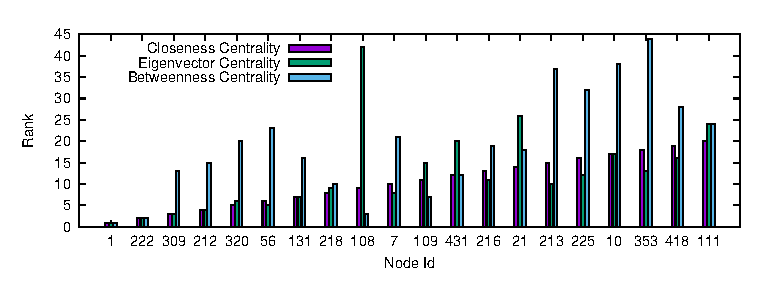
\includegraphics[width=1\textwidth]{figures/social-result_closeness.eps}
    \caption{Rank comparison for top 20 nodes ranked on closeness centrality with other centrality scores.}
    \label{fig:social-result-closeness}
\end{figure*}

\begin{figure*}[ht]
    \centering
    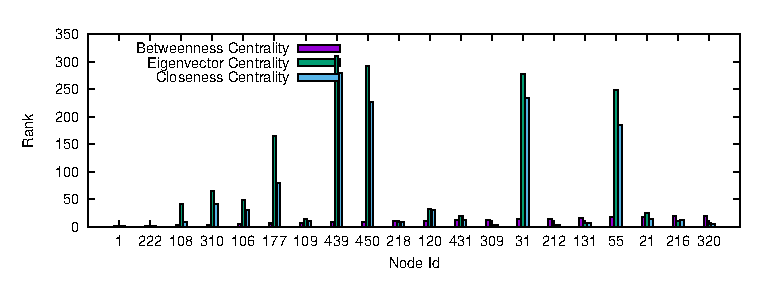
\includegraphics[width=1\textwidth]{figures/social-result_betweenness.eps}
    \caption{Rank comparison for top 20 nodes ranked on betweenness centrality with other centrality scores.}
    \label{fig:social-result-betweenness}
\end{figure*}

\paragraph{Data Collection}
For our experiments, we have collected Facebook ego network data for
the authors using facebook app "Give me my data"~\cite{givememydata}.
We also called for volunteers to give their data and verify the
results as they know the ground truth data.  For our experiment we
have assigned ids to each user in the data for privacy reasons. 

\paragraph{Results}
We picked assigned each nodes a rank based on the centrality score.
The nodes with higher importance score were ranked accordingly, 1
being the highest rank and $n$ being the lowest rank.  The ego in the
network always gets rank 1.  We then picked top 20 ranked nodes
according to each centrality score, and then compared how much rank
increment or decrement each nodes got in other measures of centrality
scores.

Figure~\ref{fig:social-result-eigen} shows the rank gain or lose for
top 20 nodes for eigenvector centrality scores when compared to other
centrality measures.  Here we can see that node 222, has the same rank
for all the three measures.  So, it shows that a node if it is really
important, remains important irrespective of centrality indicator.  We
can also see that there is not much gain or lose in rank when compared
to closeness centrality.  Node 109 gains a better rank when measured
on different centrality indicators.  But for all other nodes there is
significant drop in rank, when compared to betweenness centrality.

Figure~\ref{fig:social-result-closeness} shows the rank gain or lose for
top 20 nodes for closeness centrality scores when compared to other
centrality measures.  Here we can see that there is significant
overlap in top 20 nodes for closeness centrality and eigenvector
centrality.  Almost 15 nodes out of 20 are common for both the scales.
But when compared to betweenness centrality there is not much overlap.
But still the maximum drop to rank is not more than 45, that is less
than 10\% of the total nodes, 508.  This tells
that nodes that are important according to eigenvector centrality or
closeness centrality measures are really important nodes.  But when we
see the top 20 important nodes for betweenness centrality, see
figure~\ref{fig:social-result-betweenness}, nodes that rank high on
this score, are not among the high ranked nodes on the other
centrality indicators.  Betweenness centrality finds completely
different important nodes.  Some of these nodes are relatively less
important nodes in context of whole network, but these nodes work as a
bridge between two communities in the graph.  That is why these nodes
score high on betweenness centrality but low on other centrality
measures.

%%%%%%%%%%%%%%%%%%%%%%%%%%%%%%%%%%%%%%%%%%%%%%%%%%%%%%%%%%%%%%%%%%%%%%%%%%%%%%
% Table(s) for results of current experiments
%%%%%%%%%%%%%%%%%%%%%%%%%%%%%%%%%%%%%%%%%%%%%%%%%%%%%%%%%%%%%%%%%%%%%%%%%%%%%%

\begin{table*}[th]
\small
\centering
%\begin{tabularx}{\linewidth}{|c|c|c|c|c|c|c|X|}

\begin{tabular}{ c|c|c|c|c|c|c|c|c| }
  \cline{2-9}
  & 
  \multicolumn{2}{c}{\textbf{$u_{1}$}} &
  \multicolumn{2}{|c}{\textbf{$u_{2}$}} &
  \multicolumn{2}{|c}{\textbf{$u_{3}$}} &
  \multicolumn{2}{|c|}{\textbf{root}}  \\
  \cline{2-9}
  \multicolumn{1}{c|}{} &
  with & without & with & without & with & without & with & without\\
  \multicolumn{1}{c|}{} &
  change & changes & changes & changes & changes & changes & changes &
  changes\\
  \hline
  \multicolumn{1}{|c|}{\textbf{create file}}
  & Y & Y & N & Y & N & Y & N & Y \\
  \hline
  \multicolumn{1}{|c|}{\textbf{create dir}}
  & Y & Y & N & Y & N & Y & N & Y \\
  \hline
  \multicolumn{1}{|c|}{\textbf{remove file}}
  & Y & Y & N & Y & N & Y & N & Y \\
  \hline
  \multicolumn{1}{|c|}{\textbf{remove dir}}
  & Y & Y & N & Y & N & Y & N & Y \\
  \hline
  \multicolumn{1}{|c|}{\textbf{create symlink}}
  & Y & Y & N & Y & N & Y & N & Y \\
  \hline
  \multicolumn{1}{|c|}{\textbf{read symlink}}
  & Y & Y & N & Y & N & Y & N & Y \\
  \hline
  \multicolumn{1}{|c|}{\textbf{write symlink}}
  & Y & Y & N & Y & N & Y & N & Y \\
  \hline
  \multicolumn{1}{|c|}{\textbf{create hardlink}}
  & Y & Y & N & Y & N & Y & N & Y \\
  \hline
  \multicolumn{1}{|c|}{\textbf{write hardlink}}
  & Y & Y & N & Y & N & Y & N & Y \\
  \hline
  \multicolumn{1}{|c|}{\textbf{stat}}
  & Y & Y & N & Y & N & Y & N & Y \\
  \hline
  \multicolumn{1}{|c|}{\textbf{change dir}}
  & Y & Y & N & Y & N & Y & N & Y \\
  \hline
  \multicolumn{1}{|c|}{\textbf{read file}}
  & Y & Y & N & Y & N & Y & N & Y \\
  \hline
  \multicolumn{1}{|c|}{\textbf{write file}}
  & Y & Y & N & Y & N & Y & N & Y \\
  \hline
  \multicolumn{1}{|c|}{\textbf{create tar}}
  & Y & Y & N & Y & N & Y & N & Y \\
  \hline
  \multicolumn{1}{|c|}{\textbf{untar}}
  & Y & Y & N & Y & N & Y & N & Y \\
  \hline
  \multicolumn{1}{|c|}{\textbf{make}}
  & Y & Y & N & Y & N & Y & N & Y \\
  \hline
  \multicolumn{1}{|c|}{\textbf{rename}}
  & Y & Y & N & Y & N & Y & N & Y \\
  \hline
\end{tabular}

%\end{tabularx}
\caption{\capfont Results of different file system operations for
different users, with and without the changes.}
\label{tab:results}
\end{table*}

%%%%%%%%%%%%%%%%%%%%%%%%%%%%%%%%%%%%%%%%%%%%%%%%%%%%%%%%%%%%%%%%%%%%%%%%%%%%%%
%% For Emacs:
% Local variables:
% fill-column: 70
% End:
%%%%%%%%%%%%%%%%%%%%%%%%%%%%%%%%%%%%%%%%%%%%%%%%%%%%%%%%%%%%%%%%%%%%%%%%%%%%%%
%% For Vim:
% vim:textwidth=70
%%%%%%%%%%%%%%%%%%%%%%%%%%%%%%%%%%%%%%%%%%%%%%%%%%%%%%%%%%%%%%%%%%%%%%%%%%%%%%
% LocalWords:  PEAFS PEAIO Lustre SBU HMC config


We also had run k-means clustering algorithm on the ego network for
different k values.  For k-means clustering we have used shortest path
distance between two nodes after excluding the ego from the graph as a
distance metric.  After clustering the graph, we report centroid of
each group as important nodes.  Table~\ref{tab:k-means-results} shows
the important nodes that were reported for k=5 and their rank
according to different centrality measures.   We have varied the
number of clusters for $k=3,5,7,10,12,15,17,20$ and compared the
reported nodes with the ground truth data in
Figure~\ref{fig:social-result-arvind-kmeans}.  We observed that kmeans
works best for k=15 and worst for k=3.  A size 3 ego-network is not
very practical scenario, so its results are not accurate.  Accuracy of
kmeans is more than \emph{60\%} for all other cases.

\paragraph{Comparison of accuracy}
To verify the the experimental results with the ground truth data, we
send the top 30 nodes to the users to verify how many of them are
actually important.  Then based on their response we find the accuracy
of the algorithm in terms of \% match.  In
Figure~\ref{fig:social-result-arvind} we compared the results from ego
network of \emph{Arvind} with the ground truth data.  In this we have
taken mean accuracy of k-means along with accuracy of others. It shows
that closeness and eigen-vector give similar results.  We have also
compared the verified ground truth data for all the users in
Table~\ref{tab:accuracy-of-algorithms}.  We observe that eigen-vector
centrality gives the most accurate results and it is consistent across
all ego networks.

%%%%%%%%%%%%%%%%%%%%%%%%%%%%%%%%%%%%%%%%%%%%%%%%%%%%%%%%%%%%%%%%%%%%%%%%%%%%%%
%% For Emacs:
% Local variables:
% fill-column: 70
% End:
%%%%%%%%%%%%%%%%%%%%%%%%%%%%%%%%%%%%%%%%%%%%%%%%%%%%%%%%%%%%%%%%%%%%%%%%%%%%%%
%% For Vim:
% vim:textwidth=70
%%%%%%%%%%%%%%%%%%%%%%%%%%%%%%%%%%%%%%%%%%%%%%%%%%%%%%%%%%%%%%%%%%%%%%%%%%%%%%
% LocalWords:
